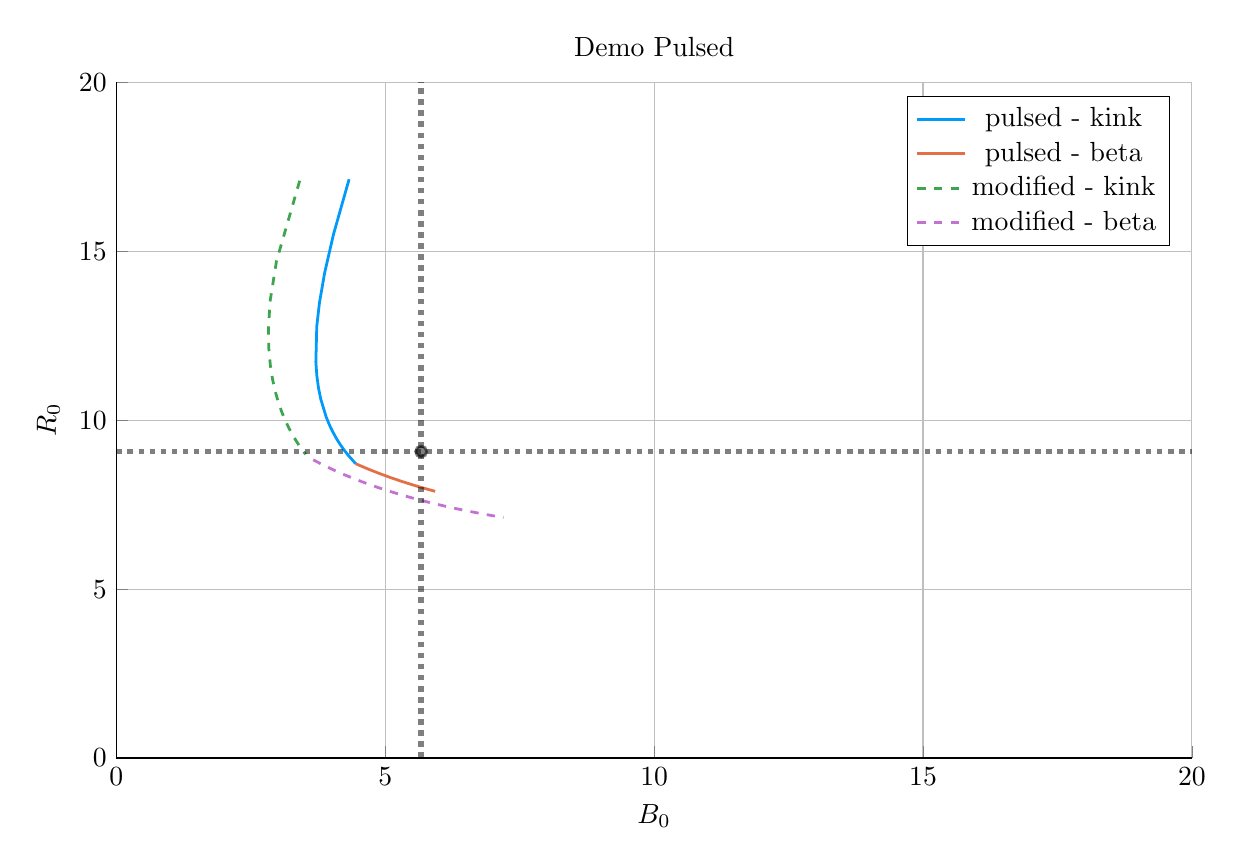
\begin{tikzpicture}[]
\begin{axis}[height = {101.6mm}, ylabel = {$R_0$}, title = {Demo Pulsed}, xmin = {0.0}, xmax = {20.0}, ymax = {20.0}, xlabel = {$B_0$}, {unbounded coords=jump, scaled x ticks = false, xticklabel style={rotate = 0}, xmajorgrids = true, xtick = {0.0,5.0,10.0,15.0,20.0}, xticklabels = {0,5,10,15,20}, xtick align = inside, axis lines* = left, scaled y ticks = false, yticklabel style={rotate = 0}, ymajorgrids = true, ytick = {0.0,5.0,10.0,15.0,20.0}, yticklabels = {0,5,10,15,20}, ytick align = inside, axis lines* = left,     xshift = 0.0mm,
    yshift = 0.0mm,
    axis background/.style={fill={rgb,1:red,1.00000000;green,1.00000000;blue,1.00000000}}
, colorbar style={title=}}, ymin = {0.0}, width = {152.4mm}]\addplot+ [color = {rgb,1:red,0.00000000;green,0.60560316;blue,0.97868012},
draw opacity=1.0,
line width=1,
solid,mark = none,
mark size = 2.0,
mark options = {
    color = {rgb,1:red,0.00000000;green,0.00000000;blue,0.00000000}, draw opacity = 1.0,
    fill = {rgb,1:red,0.00000000;green,0.60560316;blue,0.97868012}, fill opacity = 1.0,
    line width = 1,
    rotate = 0,
    solid
}]coordinates {
(4.327031075670194, 17.134796748649162)
(4.038214026054326, 15.511755022601415)
(3.8713719163129245, 14.355562963913712)
(3.7758613845615545, 13.476675762289453)
(3.7257856761317214, 12.778294295391971)
(3.7090473695925437, 11.723065749829066)
(3.727711597554826, 11.30970201784727)
(3.7586131667481433, 10.94971275897184)
(3.799052518631718, 10.632190690377048)
(3.901290136389271, 10.09455415135144)
(3.960577465316514, 9.863813619410237)
(4.0241209645210345, 9.653307397969705)
(4.0912717805663785, 9.460162902699798)
(4.161514602943343, 9.28206292757184)
(4.2344343960723005, 9.117114543572253)
(4.309692554546368, 8.963753917462126)
(4.450417240491067, 8.712493965092264)
};
\addlegendentry{pulsed - kink}
\addplot+ [color = {rgb,1:red,0.88887350;green,0.43564919;blue,0.27812294},
draw opacity=1.0,
line width=1,
solid,mark = none,
mark size = 2.0,
mark options = {
    color = {rgb,1:red,0.00000000;green,0.00000000;blue,0.00000000}, draw opacity = 1.0,
    fill = {rgb,1:red,0.88887350;green,0.43564919;blue,0.27812294}, fill opacity = 1.0,
    line width = 1,
    rotate = 0,
    solid
}]coordinates {
(4.450417240491067, 8.712493965092264)
(4.490148631384312, 8.684308742646298)
(4.692490181445514, 8.547262773806349)
(4.8960344619053355, 8.41947837460442)
(5.100651132702229, 8.30014929484307)
(5.306202822090688, 8.188581738801314)
(5.512545696627038, 8.084175191078112)
(5.719530043226767, 7.986407002697611)
(5.927000883375481, 7.894819882619234)
};
\addlegendentry{pulsed - beta}
\addplot+ [color = {rgb,1:red,0.24222430;green,0.64327509;blue,0.30444865},
draw opacity=1.0,
line width=1,
dashed,mark = none,
mark size = 2.0,
mark options = {
    color = {rgb,1:red,0.00000000;green,0.00000000;blue,0.00000000}, draw opacity = 1.0,
    fill = {rgb,1:red,0.24222430;green,0.64327509;blue,0.30444865}, fill opacity = 1.0,
    line width = 1,
    rotate = 0,
    solid
}]coordinates {
(3.4087424183072135, 17.090884129081292)
(2.977074181068944, 14.713048632784332)
(2.8592500074202523, 13.541171522519205)
(2.827199220063259, 12.740024138753894)
(2.8339789008667826, 12.12574468151967)
(2.862412302880871, 11.626187613249266)
(2.9044598258085443, 11.205091848948229)
(2.95577893007882, 10.841432203317366)
(3.0137895352525907, 10.521822649209419)
(3.076849710218805, 10.23716073884787)
(3.1438583711612704, 9.980947801083442)
(3.214045733980633, 9.748367275345563)
(3.2868548955983727, 9.535742205343247)
(3.361871149981842, 9.340197658526863)
(3.4387778750377818, 9.15944098345979)
(3.5173279629378453, 8.991613349767409)
};
\addlegendentry{modified - kink}
\addplot+ [color = {rgb,1:red,0.76444018;green,0.44411178;blue,0.82429754},
draw opacity=1.0,
line width=1,
dashed,mark = none,
mark size = 2.0,
mark options = {
    color = {rgb,1:red,0.00000000;green,0.00000000;blue,0.00000000}, draw opacity = 1.0,
    fill = {rgb,1:red,0.76444018;green,0.44411178;blue,0.82429754}, fill opacity = 1.0,
    line width = 1,
    rotate = 0,
    solid
}]coordinates {
(3.6607028750648505, 8.825949645171955)
(3.8574448036470477, 8.664618827122876)
(4.056375867871351, 8.51434867582932)
(4.257366397480293, 8.374075613831488)
(4.460279103534801, 8.242896218794312)
(4.664969389370631, 8.12003771613466)
(4.871285596007394, 8.004834914067093)
(5.07906923307514, 7.896711937521184)
(5.288155233306219, 7.795167587687744)
(5.498372259673351, 7.699763475973523)
(5.709543087166185, 7.610114306522102)
(5.921485076209294, 7.525879840414137)
(6.134010749367255, 7.446758190646709)
(6.346928478632384, 7.372480180910637)
(6.560043285872518, 7.302804563889649)
(6.773157754368795, 7.237513941672651)
(6.986073044284746, 7.176411266758267)
(7.198590001107076, 7.119316828230052)
};
\addlegendentry{modified - beta}
\addplot+ [color = {rgb,1:red,0.00000000;green,0.00000000;blue,0.00000000},
draw opacity=0.5,
line width=2,
dotted,mark = none,
mark size = 2.0,
mark options = {
    color = {rgb,1:red,0.00000000;green,0.00000000;blue,0.00000000}, draw opacity = 0.5,
    fill = {rgb,1:red,0.00000000;green,0.00000000;blue,0.00000000}, fill opacity = 0.5,
    line width = 1,
    rotate = 0,
    solid
},forget plot]coordinates {
(0.0, 9.072)
(20.0, 9.072)
};
\addplot+ [color = {rgb,1:red,0.00000000;green,0.00000000;blue,0.00000000},
draw opacity=0.5,
line width=2,
dotted,mark = none,
mark size = 2.0,
mark options = {
    color = {rgb,1:red,0.00000000;green,0.00000000;blue,0.00000000}, draw opacity = 0.5,
    fill = {rgb,1:red,0.00000000;green,0.00000000;blue,0.00000000}, fill opacity = 0.5,
    line width = 1,
    rotate = 0,
    solid
},forget plot]coordinates {
(5.667, 0.0)
(5.667, 20.0)
};
\addplot+[draw=none, color = {rgb,1:red,0.00000000;green,0.00000000;blue,0.00000000},
draw opacity=0.5,
line width=0,
solid,mark = *,
mark size = 2.0,
mark options = {
    color = {rgb,1:red,0.00000000;green,0.00000000;blue,0.00000000}, draw opacity = 0.5,
    fill = {rgb,1:red,0.00000000;green,0.00000000;blue,0.00000000}, fill opacity = 0.5,
    line width = 1,
    rotate = 0,
    solid
},forget plot] coordinates {
(5.667, 9.072)
};
\end{axis}

\end{tikzpicture}
